\chapter{Architecture et conception technique de Harmoni}
\label{ch:conception_harmoni}

Après avoir exploré l'état de l'art des solutions BPMN existantes, ce chapitre présente la conception de \textbf{Harmoni}, l'application de modélisation et d'automatisation des processus métier BPMN développée dans le cadre de ce projet. 
L'objectif est de détailler :
\begin{itemize}
    \item l'analyse des besoins (fonctionnels et non fonctionnels),
    \item la conception fonctionnelle avec diagrammes UML,
    \item l'architecture technique et la structure des composants.
\end{itemize}

\section{Analyse des besoins}

\subsection{Besoins fonctionnels}
Les besoins fonctionnels définissent les services que doit rendre l'application Harmoni :
\begin{itemize}
    \item Permettre la modélisation graphique de processus métier en notation BPMN 2.0.
    \item Assurer la validation syntaxique et la sauvegarde des modèles.
    \item Exécuter automatiquement des workflows via un moteur BPMN.
    \item Intégrer les processus automatisés aux systèmes documentaires existants de Kairos.
    \item Fournir un tableau de bord de monitoring en temps réel des processus exécutés.
    \item Gérer les utilisateurs, rôles et droits d’accès (gestionnaires de processus, utilisateurs finaux).
\end{itemize}

\subsection{Besoins non fonctionnels}
Les besoins non fonctionnels fixent les contraintes de performance, de sécurité et de maintenabilité :
\begin{itemize}
    \item \textbf{Performance} : temps de réponse inférieur à 2 secondes pour les opérations critiques.
    \item \textbf{Scalabilité} : support de plusieurs centaines d’instances de processus simultanées.
    \item \textbf{Sécurité} : authentification par JWT, communications chiffrées en HTTPS.
    \item \textbf{Interopérabilité} : respect du standard BPMN 2.0 et API REST pour intégration.
    \item \textbf{Fiabilité} : gestion robuste des erreurs et reprise après panne.
    \item \textbf{Ergonomie} : interface intuitive adaptée aux utilisateurs métier non techniques.
\end{itemize}

\section{Conception fonctionnelle}

\subsection{Diagramme de cas d’utilisation}
La figure~\ref{fig:uc_bpmn_app} présente les principaux acteurs et cas d'utilisation de la plateforme.  
\begin{figure}[h]
    \centering
    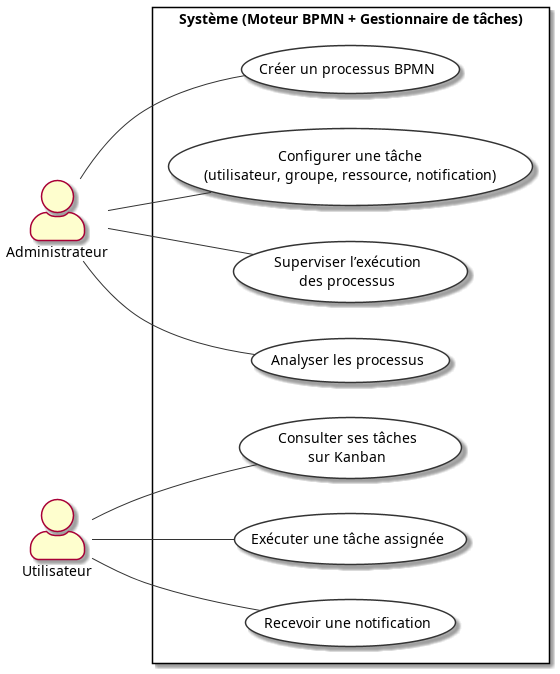
\includegraphics[width=0.5\textwidth]{Images/usecase.png}
    \caption{Diagramme de cas d'utilisation — Application BPMN}
    \label{fig:uc_bpmn_app}
\end{figure}

\subsection{Diagramme de classes}
Le diagramme de classes met en évidence les entités principales (Processus, Tâche, Utilisateur, Document, Notification, etc.) et leurs relations (voir Figure~\ref{fig:class_bpmn_app}).  
% \begin{figure}[h]
%     \centering
%     \includegraphics[width=0.9\textwidth]{Images/class.png}
%     \caption{Diagramme de classes — Modèle conceptuel de Harmoni}
%     \label{fig:class_bpmn_app}
% \end{figure}

\subsection{Diagramme de séquence}
La figure~\ref{fig:seq_exec_bpmn} illustre une séquence représentative d'exécution d'un processus BPMN par un utilisateur, depuis la modélisation jusqu’au monitoring.
\begin{figure}[h]
    \centering
    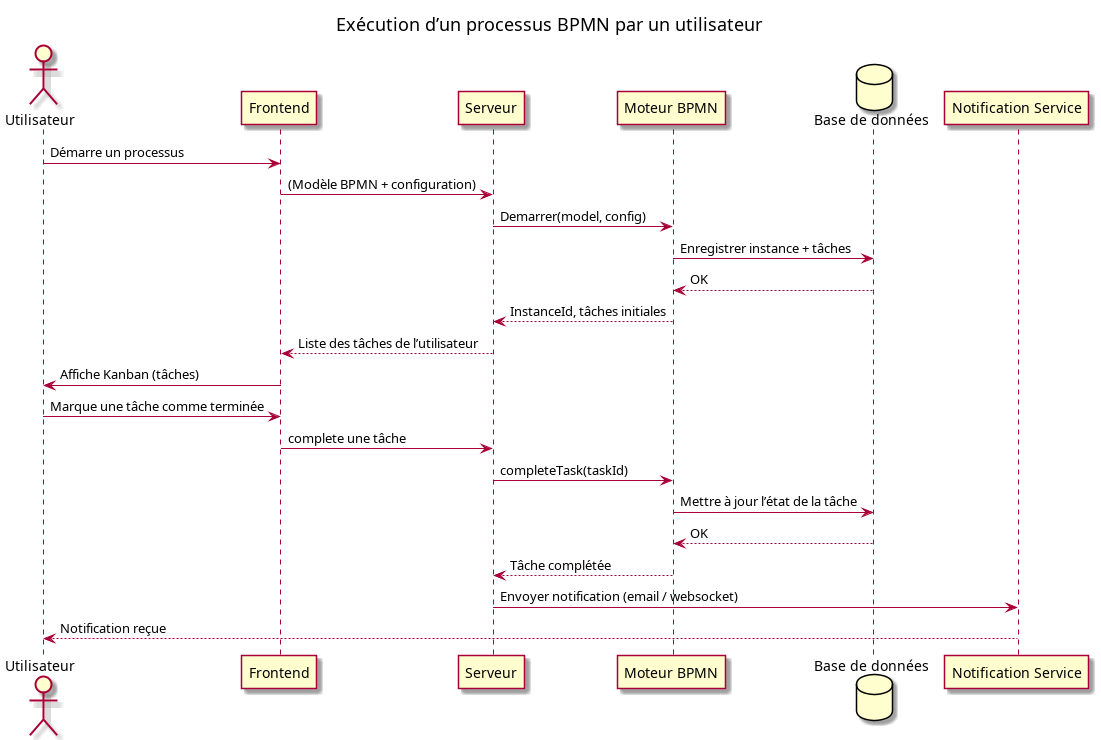
\includegraphics[width=0.95\textwidth]{Images/sequence.png}
    \caption{Diagramme de séquence — Exécution d’un processus BPMN par un utilisateur}
    \label{fig:seq_exec_bpmn}
\end{figure}

\section{Structure des composants et dépendances}

\subsection{Schéma directeur de Harmoni}
Cette section présente l'architecture globale de Harmoni et les flux principaux entre les composants.
\begin{figure}[h]
    \centering
    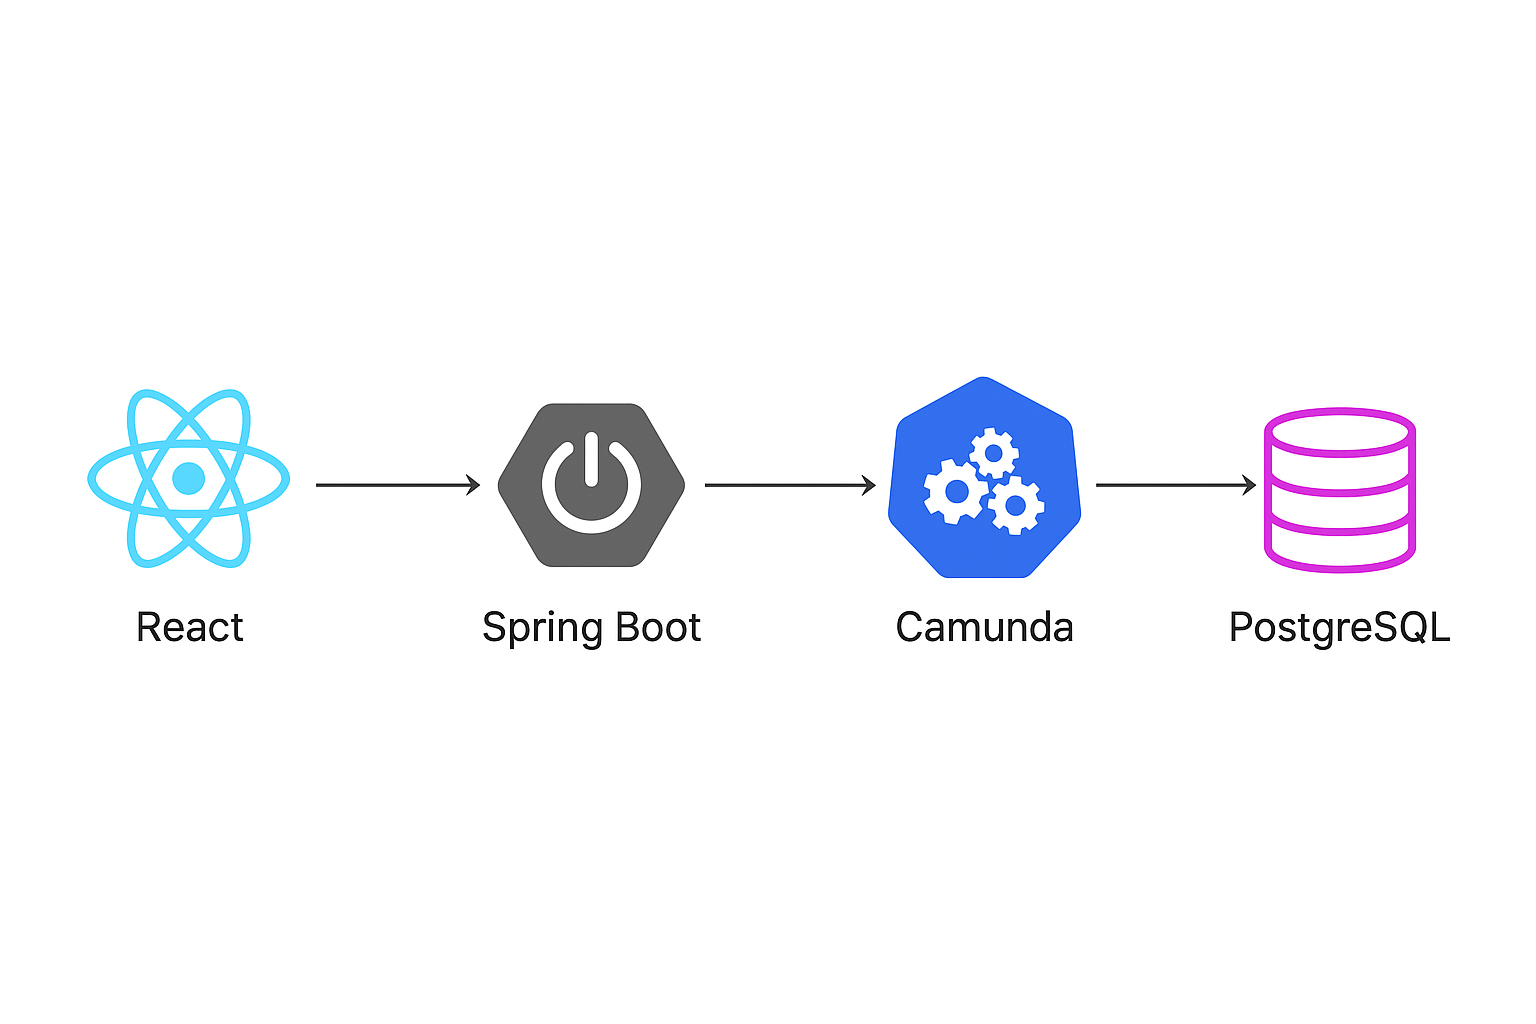
\includegraphics[width=0.8\textwidth]{Images/Architecture.png}
    \caption{Architecture globale de Harmoni}
    \label{fig:harmoni_global_architecture}
\end{figure}

\subsection{Choix de l’architecture}
Cette sous-section détaille les couches (React, API Spring Boot, Moteur BPMN, Intégrations) et leurs responsabilités.

\subsection{Flux de données et interactions}
Synthèse des échanges entre frontend, API, moteur BPMN et systèmes documentaires.

\section{Implémentation technique}

\subsection{Le cœur logique de Harmoni}
(== ton texte existant sur l’architecture Spring Boot, API REST, sécurité, moteur BPMN ==)

\subsection{L’interface utilisateur React}
(== ton texte existant sur l’éditeur BPMN, React, monitoring, etc. ==)

---
